%%%
%  File: chapter1.tex
%  Project: rp-doc
%  Author: Javier Reyes
%  Created on: 08.09.2018
%  
%  Last modified: 08.09.2018
%  Modified by: Javier Reyes (javier.reyes.g@gmail.com)
%  
%  MIT License
%  
%  Copyright (c) 2018 Javier Reyes
%  
%  Permission is hereby granted, free of charge, to any person obtaining a copy of
%  this software and associated documentation files (the "Software"), to deal in
%  the Software without restriction, including without limitation the rights to
%  use, copy, modify, merge, publish, distribute, sublicense, and/or sell copies
%  of the Software, and to permit persons to whom the Software is furnished to do
%  so, subject to the following conditions:
%  
%  The above copyright notice and this permission notice shall be included in all
%  copies or substantial portions of the Software.
%  
%  THE SOFTWARE IS PROVIDED "AS IS", WITHOUT WARRANTY OF ANY KIND, EXPRESS OR
%  IMPLIED, INCLUDING BUT NOT LIMITED TO THE WARRANTIES OF MERCHANTABILITY,
%  FITNESS FOR A PARTICULAR PURPOSE AND NONINFRINGEMENT. IN NO EVENT SHALL THE
%  AUTHORS OR COPYRIGHT HOLDERS BE LIABLE FOR ANY CLAIM, DAMAGES OR OTHER
%  LIABILITY, WHETHER IN AN ACTION OF CONTRACT, TORT OR OTHERWISE, ARISING FROM,
%  OUT OF OR IN CONNECTION WITH THE SOFTWARE OR THE USE OR OTHER DEALINGS IN THE
%  SOFTWARE.
%%%

\chapter{DAEbot Environment} \label{chapter1}

The DAEbot project stands for Distributed Architectures Evaluation robot, a modular system that
allows different approaches for distributed hardware and software architectures to be tested
\cite{Wiki}.

The robot is designed and built with common hardware (evaluation boards and popular
sensors-actuators), so that it can be easily replaced or tested with different devices, as well as
test different software solutions or methodologies. Physically, the robot represents a layered
structure, to resemble the software architecture approach that is used, which is based in the OCM
software architecture.

\section{OCM Architecture}

Typical mechatronic systems complexity grows exponentialy with every new technological step, which
requieres a careful process of defining the right architecture for mechatronic systems. On this base
concept, the goal for the DAEbot architecture is graphically represented in the figure
\ref{fig:ocm-dae}.

\begin{figure}[htp]
	\centering
	\begin{subfigure}{0.5\textwidth}
		\centering
		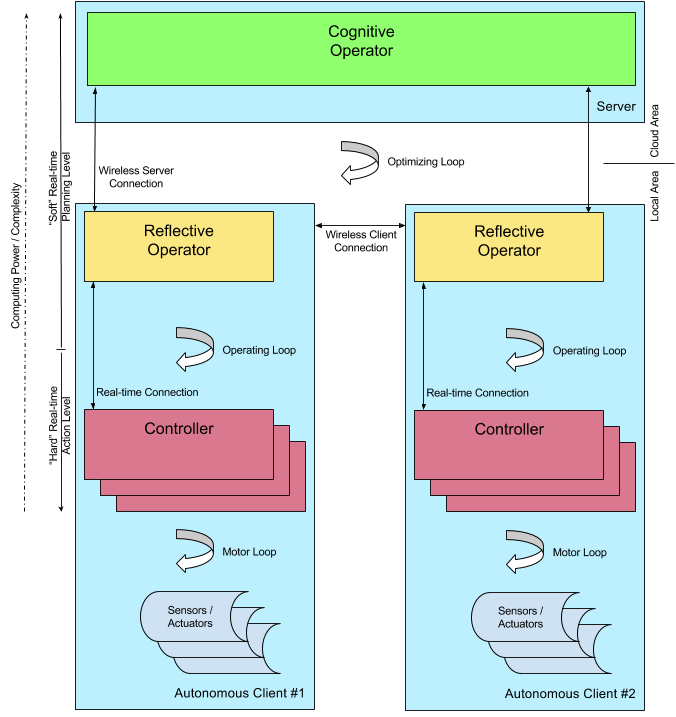
\includegraphics[width=\textwidth]{ocm-architecture.png}
		\caption{OCM model.} \label{fig:ocm-architecture}
	\end{subfigure}%
	\begin{subfigure}{0.5\textwidth}
		\centering
		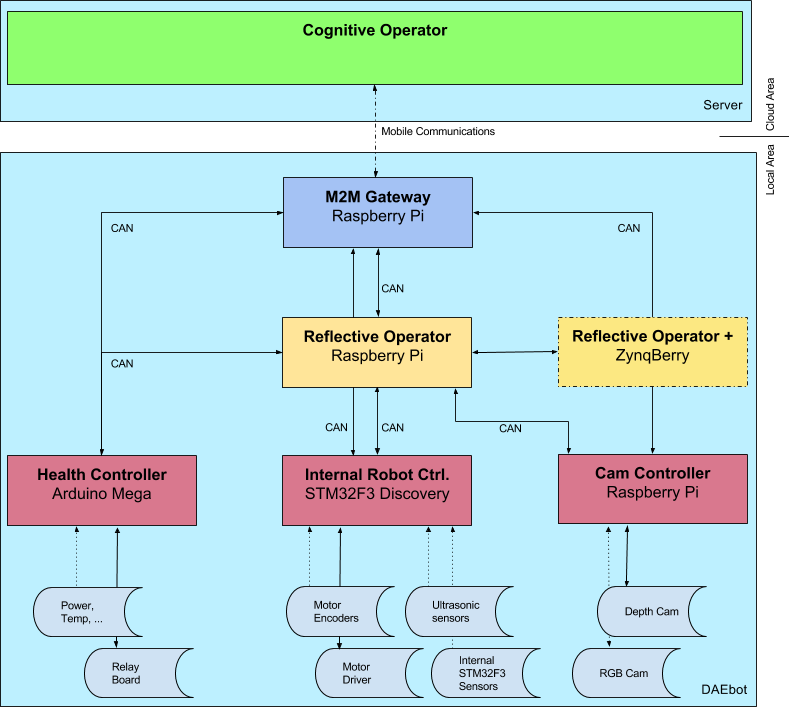
\includegraphics[width=\textwidth]{dae-architecture.png}
		\caption{DAEbot model.} \label{fig:dae-architecture}
	\end{subfigure}%
	\caption{OCM software architectural model, from \cite{Wiki}.} \label{fig:ocm-dae}
\end{figure}%

The OCM structure is based on the work of the Mechatronics Laboratory Paderborn as a hierarchical
structure for mechatronics systems \cite{Lueckel2001}. This structure defines three different layers
that allows the clear seaparation of controllers, considering the real-time characteristics, and
therefore allowing a more comprehensive development process. The DAEbot defined structure related to
the OCM architecture can be seen in figure \ref{fig:dae-architecture}.

Given the modular architecture, the design and develoment of each of the elements in the system can
be modularized and worked independently, under the guidelines of the structure.

\subsection*{Controller Layer}

This is the lowest level layer, where the traditional controller is defined as a traditional control
loop, usually based on a mathematical model. This way the controller gains flexibility in terms of
the configuration parameters, and can be individually simulated and tested (XiL), allowing different
operation modes which will be \textit{operated} from the next layer.

\subsection*{Reflective Operator Layer}

On this layer, the monitoring and control is implemented, and even allow communication with other
systems in a network.

\subsection*{Cognitive Operator}

For more complex systems, that need coordination/communication interactions or learning algorithms,
the Cognitive layer expands the functionality.

\section{Zynqberry 726 Single Board Computers}

The zynqberry board, with its FPGA capababilities, is considered a second operator with the
expectation of evaluating a true parallel application performance inside the OCM architecture. The
communication from and to the main Reflective Operator (Raspberry Pi) and the Controllers is
provided by CAN bus, with an optional link via Ethernet for high data payloads.

\begin{figure}[htp]
	\centering
	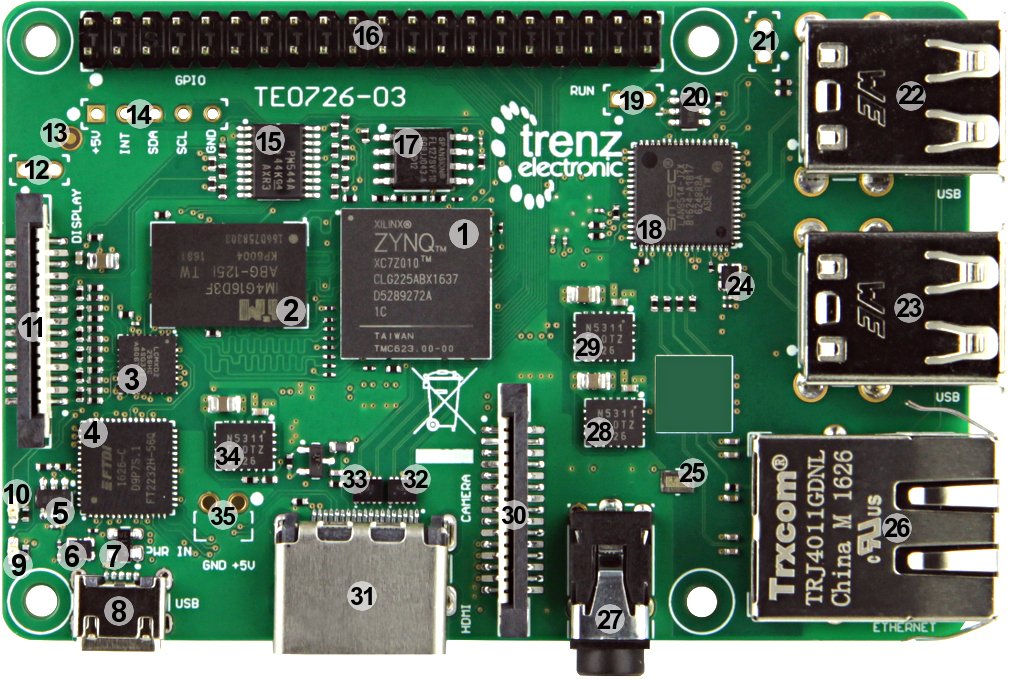
\includegraphics[width=0.5\textwidth]{zynqberry-top.png}
	\caption{Top view of the Znyqberry board, from \cite{zynq-main}.} \label{fig:znyqtop}
\end{figure}

\subsection{Board Peripherals}

The Zynqberry board, developed by the company Trenz Electronic GmbH, is a SoM (System on Module)
based on the Xilinx All Programmable Zynq-700 SoC (XC7Z010) along with standar peripherials in an
industrial-grade Raspberry Pi form factor. Some of the most relevant features are listed below
\cite{zynq-main}:

\begin{itemize}
	\item Xilinx Zynq XC7Z010-1CLG225C
	\begin{itemize}
		\item 128 MByte DDR3L SDRAM
		\item 16 MByte Flash
	\end{itemize}
	\item Raspberry Pi Model 2 form factor
	\item LAN9514 USB hub with Ethernet
	\begin{itemize}
		\item 4 x USB with power switches
		\item 100 MBit Ethernet RJ45
	\end{itemize}
	\item Micro SD cad slot
	\item HAT header with 26 I/O's
	\item HDMI Type A
	\item DSI Connector (display)
	\item CSI-2 Connector (camera)
	\item Micro USB
	\begin{itemize}
		\item Power input
		\item USB UART
		\item JTAG ARM- and FPGA-Debug
	\end{itemize}
	\item 3.5 mm audio plug (PWM audio output only)
\end{itemize}

\begin{figure}[htp]
	\centering
	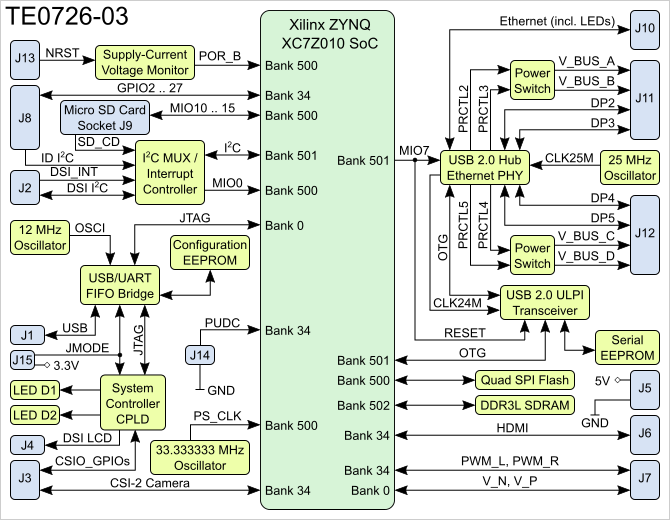
\includegraphics[width=0.7\textwidth]{zynq-block-diagram.png}
	\caption{Block diagram of the Zynqberry 726, from \cite{zynq-trm}.}
	\label{fig:zynqblock}
\end{figure}

The physical device used in this project corresponds to the version 02 of the product, despite the
fact that the manufacturer holds a newer 03 version. This needs to be considered during any
reference consultation.

\section{Zynq-7000 System-on-Chip}\label{zynq7-soc}

The heart of the Zynqberry SBC is one of the Zynq-7000 All Programmable System-on-Chip devices, with
the product name XC7Z010-1CLG225C. This device offers a dual-core ARM Cortex-A9, defined in the
architecture as Processing System (PS), as well as a Xilinx Programmable Logic (PL) based on a 28 nm
High-Performance Low-Power technolgy, together in a single chip. This combination helps to fulfill
high-speed logic, arithmetic and data flow functionality, together with software routines and
Operative Systems supported by lower layer drivers for the hardware system.

\begin{figure}[htp]
	\centering
	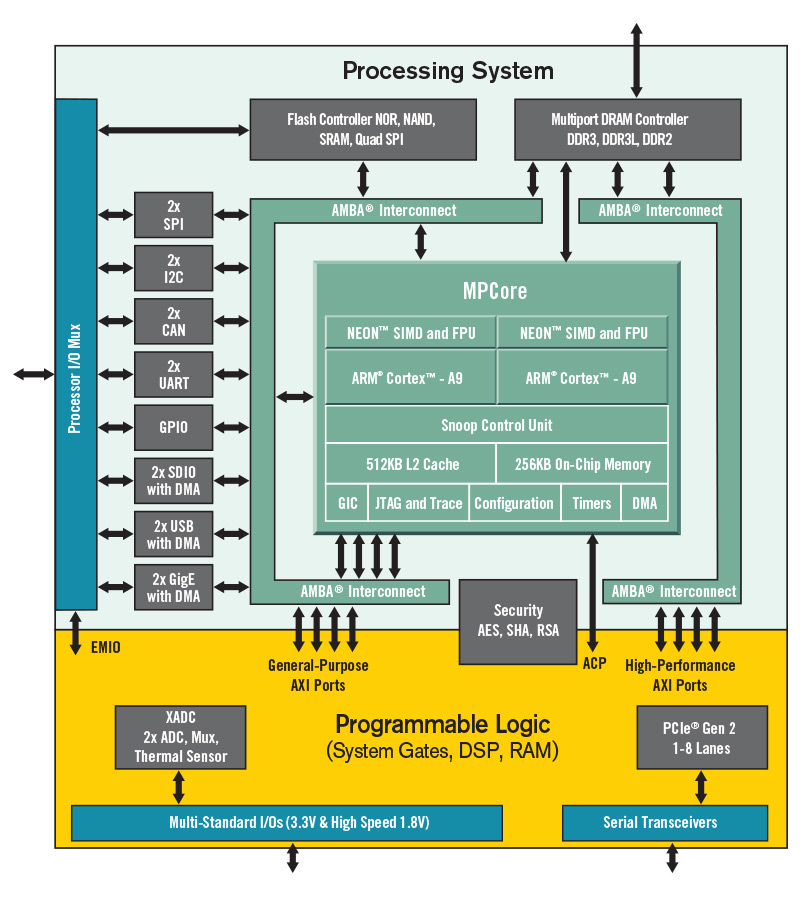
\includegraphics[width=0.6\textwidth]{zynq-arch-diag.png}
	\caption{Zynq XC7Z010 architectural diagram, from \cite{DS190}.} \label{fig:zynq-arch-diag}
\end{figure}

The Zynq architecture allows the interconnection between PS  and PL signals, offering higher levels
of performance compared to two-chip solutions, thanks to the industry standard AXI interfaces
\cite{Crokett2014}. The main system is considered to be the PS, as it is the first one to boot up,
and has the responsability to configure the PL (either during boot, or at any future moment) via a
bitstream.

The PL provides Configurable Logic Blocks (CLB), port and width configurable block RAM, DSP slices
with 25x18 multiplier, 48-bit accumulator and pre-adder, user configurable analog-to-digital
convertor (XADC), Clock Management Tiles (CMT), and a configuration block with 256-bit AES for
decryption and SHA for authentication. External connections for peripheral IO ports in the PS are
mainly handled through a multiplexed module (MIO) up to 54 pins, but can also be redirected through
the PL domain (EMIO).

Several options are posible for the boot process, as it goes through the ROM and a First-Stage
Bootloader (FSBL), which means it can be adjusted to the start-up needs of the application. The
device provide secure and non-secure boot configurations, even for the PL bitstream configuration
(which need to be powered on, given that the AES decryption and SHA authentication blocks are
located in the PL). In constrast, power on the PL can be shutdown to reduce power consumption, as
well as the clocks signals can be dynamically slowed down or turned off if needed.

It is important to remark that the specific device that is found in the Zynqberry 0726-02M has a
special hardware difference with respect to the rest of the family:
\begin{quote} 
	\centering 
	\say{The 7Z007s single core and 7Z010 dual-core CLG225 devices have a limited number of pins
	(225). This reduces the capability of the MIO, DDR and XADC subsystems}
\end{quote}
\textbf{7Z007s and 7Z010 CLG225 constraints:}
\begin{itemize}
	\item 32 MIO pins.
	\item 16 DDR data.
	\item Four pairs of XADC signals.
\end{itemize}

More detailed technical reference information can be found in \cite[p.~30]{UG585}.

\subsection{Processing System}

The Processing System (PS) present on the Zynq chip is a 'hard' processor (existent in silicon on
the device), as oposed to the alternative 'soft' processor like Xilinx MicroBlaze (formed by
progammable logic elements). Given enough resources in the PL, one -or more- MicroBlaze processors
can be added in conjunction to the ARM PS. 

The PS provides high performance charactersitics as (more details in \cite[p.~32]{UG585}):
\begin{itemize}
	\item Dual core with asymmetrical or symmetrical multiprocessing.
	\item 32 kB instrcution and data L1 cache memory.
	\item 512 kB of shareable L2 cache memory.
	\item Accelerator Coherency Port (ACP) from PL to PS.
	\item 256 kB of on-chip SRAM.
	\item DMA controller.
	\item General Interrupt Controller.
	\item Watchdog timer and Triple Timer Counter.
\end{itemize}

Each core of the ARM PS provides a NEON Media Processing Engine (MPE) and a Floating Point Unit
(FPU). The NEON engine takes relevance for acceleration requirements with the functionality Single
Instruction Multiple Data (SIMD), extended from the standard ARM instruction set. The computational
gain of NEON engine can be either specificaly triggered, or ensured by compiler recognition of
viable format in C code.

\begin{figure}[htp]
	\centering
	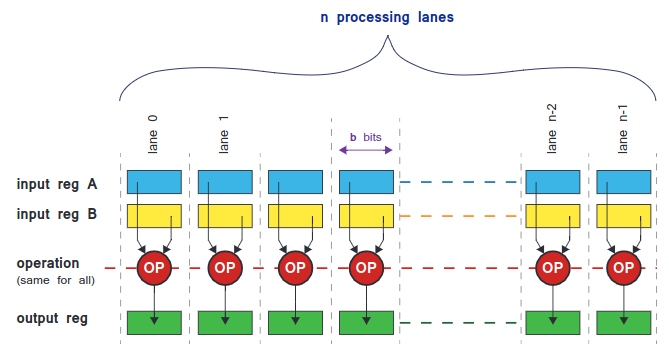
\includegraphics[width=0.7\textwidth]{neon-structure.png}
	\caption{Processing scheme for SIMD NEON engine, from \cite{Crokett2014}.}
	\label{fig:neon-structure}
\end{figure}

\subsubsection{Peripherals}

The I/O peripherals are based on industry-standards, for external data communication. The ARM PS
included in the XC7Z010 device provides among others:

\begin{itemize}
	\item GPIO - MIO, EMIO
	\begin{itemize}
		\item Two IO voltage banks
		\item Voltage level programmable per bank
	\end{itemize}
	\item SPI (x2)
	\begin{itemize}
		\item Four wire bus (MOSI, MISO, SCLK, SS)
		\item Full-duplex operation
		\item Master, Slave or Multi-master modes
		\item 50 MHz maximum external clock through MIO
		\item 128-byte read and 128-byte write FIFOs
		\item Manual or auto start data transmission
	\end{itemize}
	\item I2C (x2)
	\begin{itemize}
		\item 16-byte FIFO
		\item Programmable normal and fast bus data rate
		\item Master, Slave, and Slave-monitor modes
	\end{itemize}
	\item CAN (x2)
	\begin{itemize}
		\item ISO 11898-1, CAN 2.0A and CAN 2.0B standards
		\item Standard and extended identifier frames
		\item Up to 1 Mb/s rates
		\item Tx and Rx message FIFO with 64 depth
		\item Watermark interrupts for TxFIFO and RxFIFO
		\item Automatic re-transmission on error or arbitration loss
		\item Up to 4 acceptance filters
	\end{itemize}
	\item UART (x2)
	\begin{itemize}
		\item Programmable baud rate generator
		\item 64-byte receive and transmit FIFOs
		\item Modem control signals (CTS, RTS, DSR, RI, DCD)
	\end{itemize}
	\item SD (x2)
	\begin{itemize}
		\item Bootable SD card mode
		\item Built-in DMA
		\item Host mode only
		\item 1-bit and 4-bit data interface supported
		\item Low speed clock 0-400 kHz / Full speed clock 0-50 MHz
		\item 1kB data FIFO interface
	\end{itemize}
	\item USB (x1)
	\begin{itemize}
		\item Host, Device or OTG
		\item USB 2.9 high-speed device and controller
		\item EHCI compatible
		\item MIO pins only
	\end{itemize}
	\item Gigabit Ethernet (x2)
	\begin{itemize}
		\item RGMII interface using MIO pins and external PHY
		\item SGMII using PL GTP or GTX transceivers
		\item Built-in DAM with scatter-gather
		\item IEEE 802.3-2008 and 1588 revision 2.0
		\item Wake-on capability
	\end{itemize}
\end{itemize}

\subsection{Programmable Logic}

The Programmable Logic PL section of the XC7Z010 device is mainly composed of FPGA Logic Fabric,
along with Input/Output Blocks for interfacing. Other useful sections include RAM memory blocks, DSP
resources, an Analog-to-Digital Conversor, and Clock Management \cite[p.~23]{Crokett2014}.

\begin{figure}[htp]
	\centering
	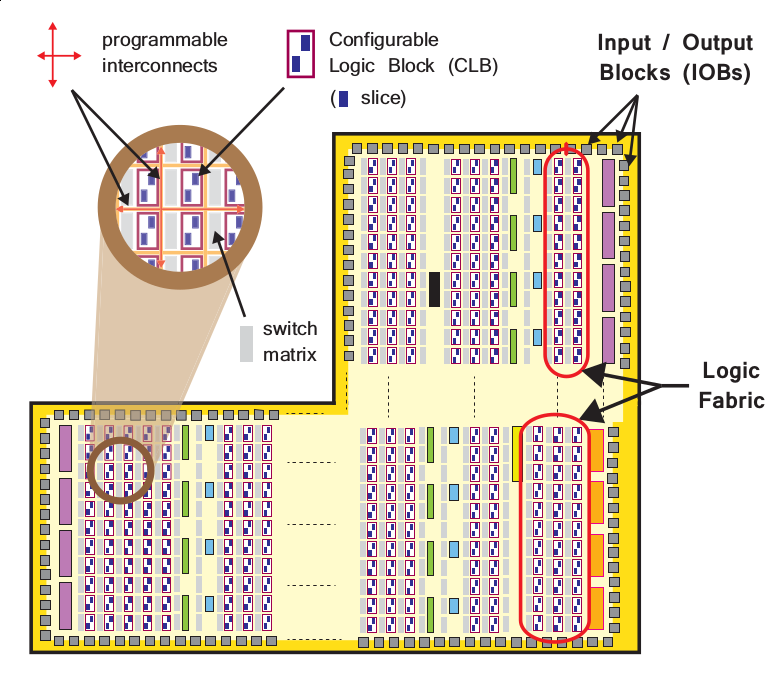
\includegraphics[width=0.7\textwidth]{fpga-compose.png}
	\caption{General purpose Logic Fabric composition, from \cite{Crokett2014}.}
	\label{fig:fpga-compose}
\end{figure}

\subsubsection{Configurable Logic Blocks}

The CLB's are the elements where the combinational and sequential logic is implemented in the Zynq
device. Includes 6-input Lookup Tables (LUT), Flip Flops (FF) and 2-D switch matrixes for each CLB.

\begin{figure}[htp]
	\centering
	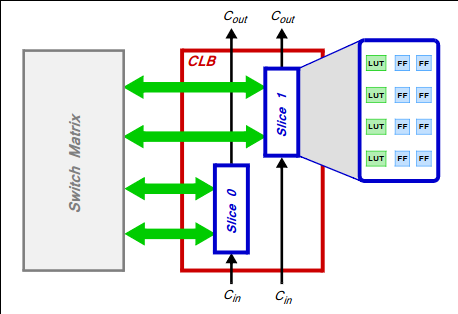
\includegraphics[width=0.7\textwidth]{fpga-clb.png}
	\caption{Configurable Logic Blocks composition, from \cite{Crokett2014}.}
	\label{fig:fpga-clb}
\end{figure}

\subsubsection{DSP Blocks}

Silicon resources available for arithmetic circuits (specially those with long wordlengths). Include
pre-adder, multiplier, and post-adder with logic unit, as shown in figure \ref{fig:fpga-dsp}.

\begin{figure}[htp]
	\centering
	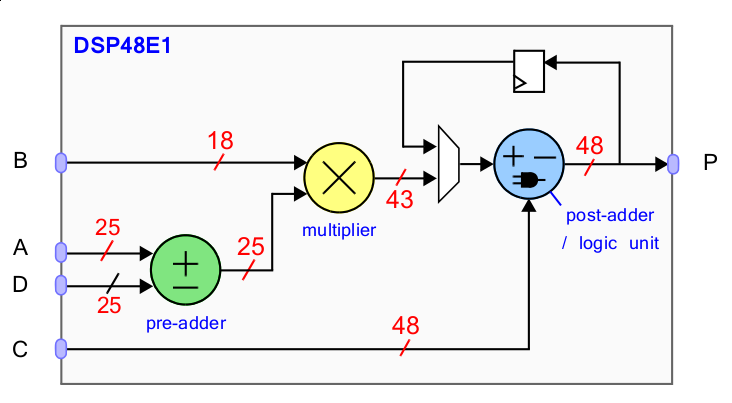
\includegraphics[width=0.5\textwidth]{fpga-dsp.png}
	\caption{Arithmetic DSP blocks composition, from \cite{Crokett2014}.}
	\label{fig:fpga-dsp}
\end{figure}

\subsubsection{RAM Blocks}

Implemented close to the DSP blocks as columns between the fabric logic, as it is fairly common that
long arithmetic tasks are performed close to one another. They can implement RAM and ROM memory
blocks, as well as FIFO buffers, up to 36 kB configurable based on a default 18-bit size word.

\begin{figure}[htp]
	\centering
	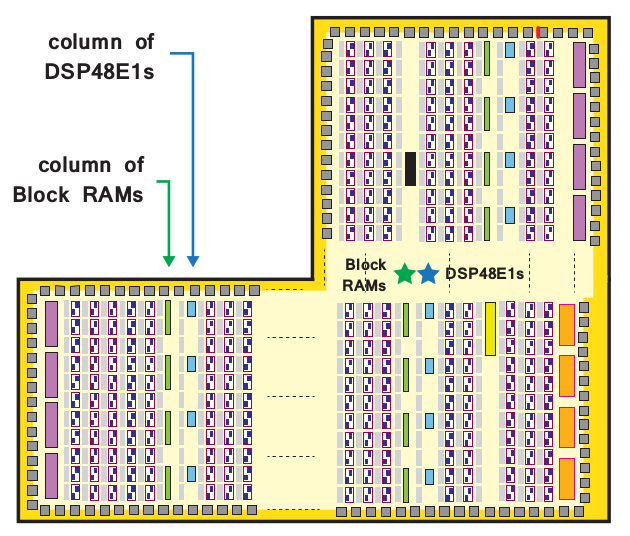
\includegraphics[width=0.5\textwidth]{fpga-ram.png}
	\caption{DSP and RAM blocks in the logic fabric, from \cite{Crokett2014}.}
	\label{fig:fpga-ram}
\end{figure}

All of this resources are usually defined to be targeted by the tools (Synthesis and
Implementation), it is always a good advice to be aware of the technological capabilities.

\subsubsection{IO Blocks}

The logical resources are surrounded by general purpose Input / Output blocks, providing connection
to the outside. This resources are organized by 50 IOB, and categorised as High Performance (HP) or
High Range (HR). HP banks are focused on 1.8V level and high-speed interfaces to memory and external
chips, whereas HR allows up to 3.3V and other IO standards.

To obtain a more detailed description for development, the Technical Reference Manual
\cite[p.~38]{UG585} offers a full detail of features and characteristics.

\subsection{PS-PL Interfaces}

\subsubsection*{AXI Interconnect}

The main feature of the Zynq architecture is the ability to use both PS and PL in an integrated
system. For this, the \textit{AXI Interconnect} is a key element, as it forms a bridge between the
two units. This standard for \textbf{A}dvanced E\textbf{X}tensible \textbf{I}nterface (in its
current version, AXI4) is part of ARM AMBA 3.0 open standard, described as \textit{"the de facto
standard for for on-chip communication"} \cite{Crokett2014}.

There are three different bur protocols for AXI, depending of the specific connection properties:

\begin{itemize}
	\item AXI4: For memory-mapped links, with highest performance. An address is suplied, and a
	burts of up to 256 data words can follow.
	\item AXI4-Lite: Simplified link (an address and a single data word) for only one transfer per
	connection, also memory-mapped.
	\item AXI4-Stream: For high-speed streaming data, supports burst transfers without size
	restriction. No address mechanism, best suited to direct data flow between source and
	destination, without memory-mapping.
\end{itemize}

Behind each AXI Intercconnect, there are several different interfaces possible in the Zynq
architecture. In the figure \ref{fig:zynq-axi-structure} can be seen the typical structure of AXI
Interconnects and Interfaces.

\begin{figure}[htp]
	\centering
	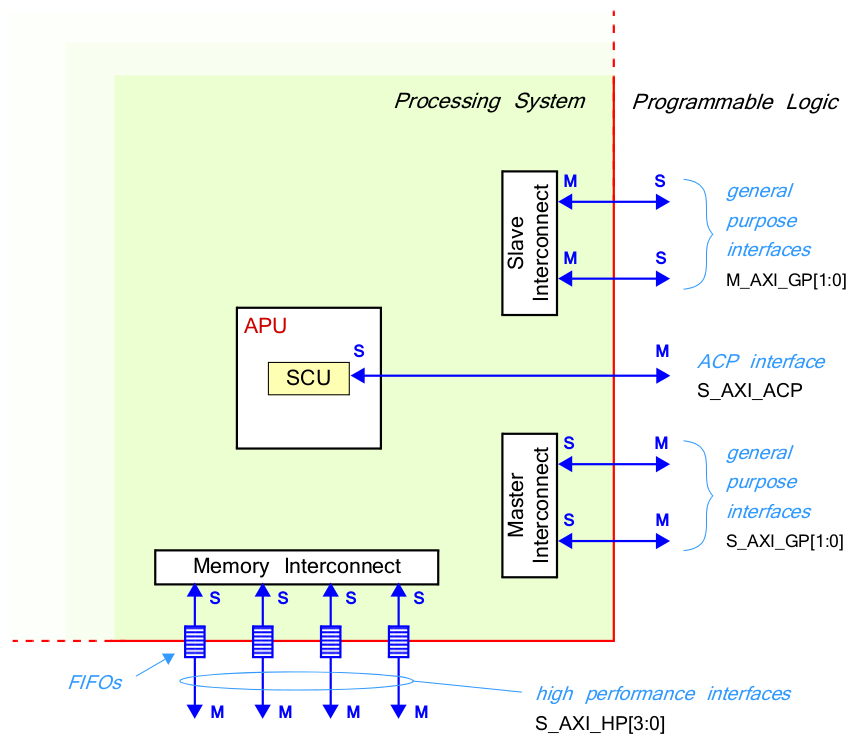
\includegraphics[width=0.5\textwidth]{zynq-axi-structure.png}
	\caption{Structure of AXI Interconnects and interfaces between PS and PL, from
	\cite{Crokett2014}.} \label{fig:zynq-axi-structure}
\end{figure}

\begin{itemize}
	\item General Purpose AXI: A 32-bt data bus, suitable for low and medium rate communitcations
	between PL and PS. The direction of the communication is dictated by the master and slave of it.
	Ps is master of two of them, and PL is master of other two.
	\item Accelerator coherency Port: A single asynchronous connection between PL and the SCU within
	the APU with a bus width of 64 bits. Used to achieve coherency between APU caches and elements
	in PL, which is the master.
	\item High Performance Port: Four HP interfaces that include FIFO buffers to handle data burst
	(read and write), and high rate communications between PL and memory elements in the PS. Data
	can be 32 or 64 bits, and the master is PL.
\end{itemize}

\subsubsection*{EMIO}

As mentioned in \ref{zynq7-soc}, the Zynq architecture includes ports for signals in the PS, which
are hard defined in the chip layout. When these connections are not enough, one can expand the ports
through the PL to external interfaces, referred to as Extended MIO.

It is important to remark that not all MIO signals can be routed through EMIO, and those who
actually can will have reduced capability. The routed signals can be either connected to external
pins of the PL (specified in an appropiate constraint file), or connect to peripherial blocks
present in the PL.

\begin{figure}[htp]
	\centering
	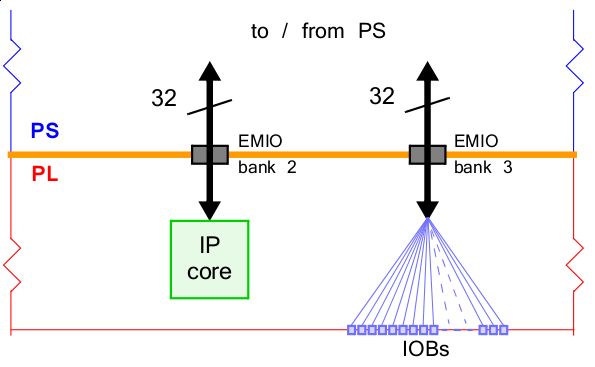
\includegraphics[width=0.5\textwidth]{emio-interface.png}
	\caption{EMIO interface usage, from \cite{Crokett2014}.} \label{fig:emio-interface}
\end{figure}
